\section{实验思路说明}

\subsection{题目1 - 基本链表操作}

这道题主要练习链表的基本操作。判断链表是否递增时,只要依次比较相邻节点就行;链表逆置用头插法最方便,不用另外开空间;克隆链表要注意深拷贝,每个节点都要重新创建。最后排序输出用了最简单的冒泡排序,虽然不是最优的,但容易理解。

\subsection{题目2 - 有序链表}

这题设计了一个自动保持有序的链表。插入新节点时要先找到合适的位置,这样整个链表就能一直保持有序。删除重复节点时,由于链表本身是有序的,重复的节点一定相邻,所以比较容易处理。区间删除用了两个指针,一前一后遍历,遇到符合条件的节点就删掉。

\subsection{题目3 - 算法设计}

这题既要写顺序表也要写链表的算法。顺序表的有序插入要把后面的元素都往后挪;删除指定值时,为了节省空间,用覆盖的方法就行。链表部分基本都是第一题和第二题思路的综合应用,主要是要注意一些细节,比如释放删除节点的空间,防止内存泄漏。

\section{代码实现中的一些注意点}

\begin{itemize}
	\item 用了模板,这样链表就能存各种类型的数据
	\item 加了头节点,这样很多操作都好写一些
	\item 删除节点时记得释放内存
	\item 尽量把代码写得清晰一点,方便以后看
\end{itemize}

\begin{figure}[H]
\centering
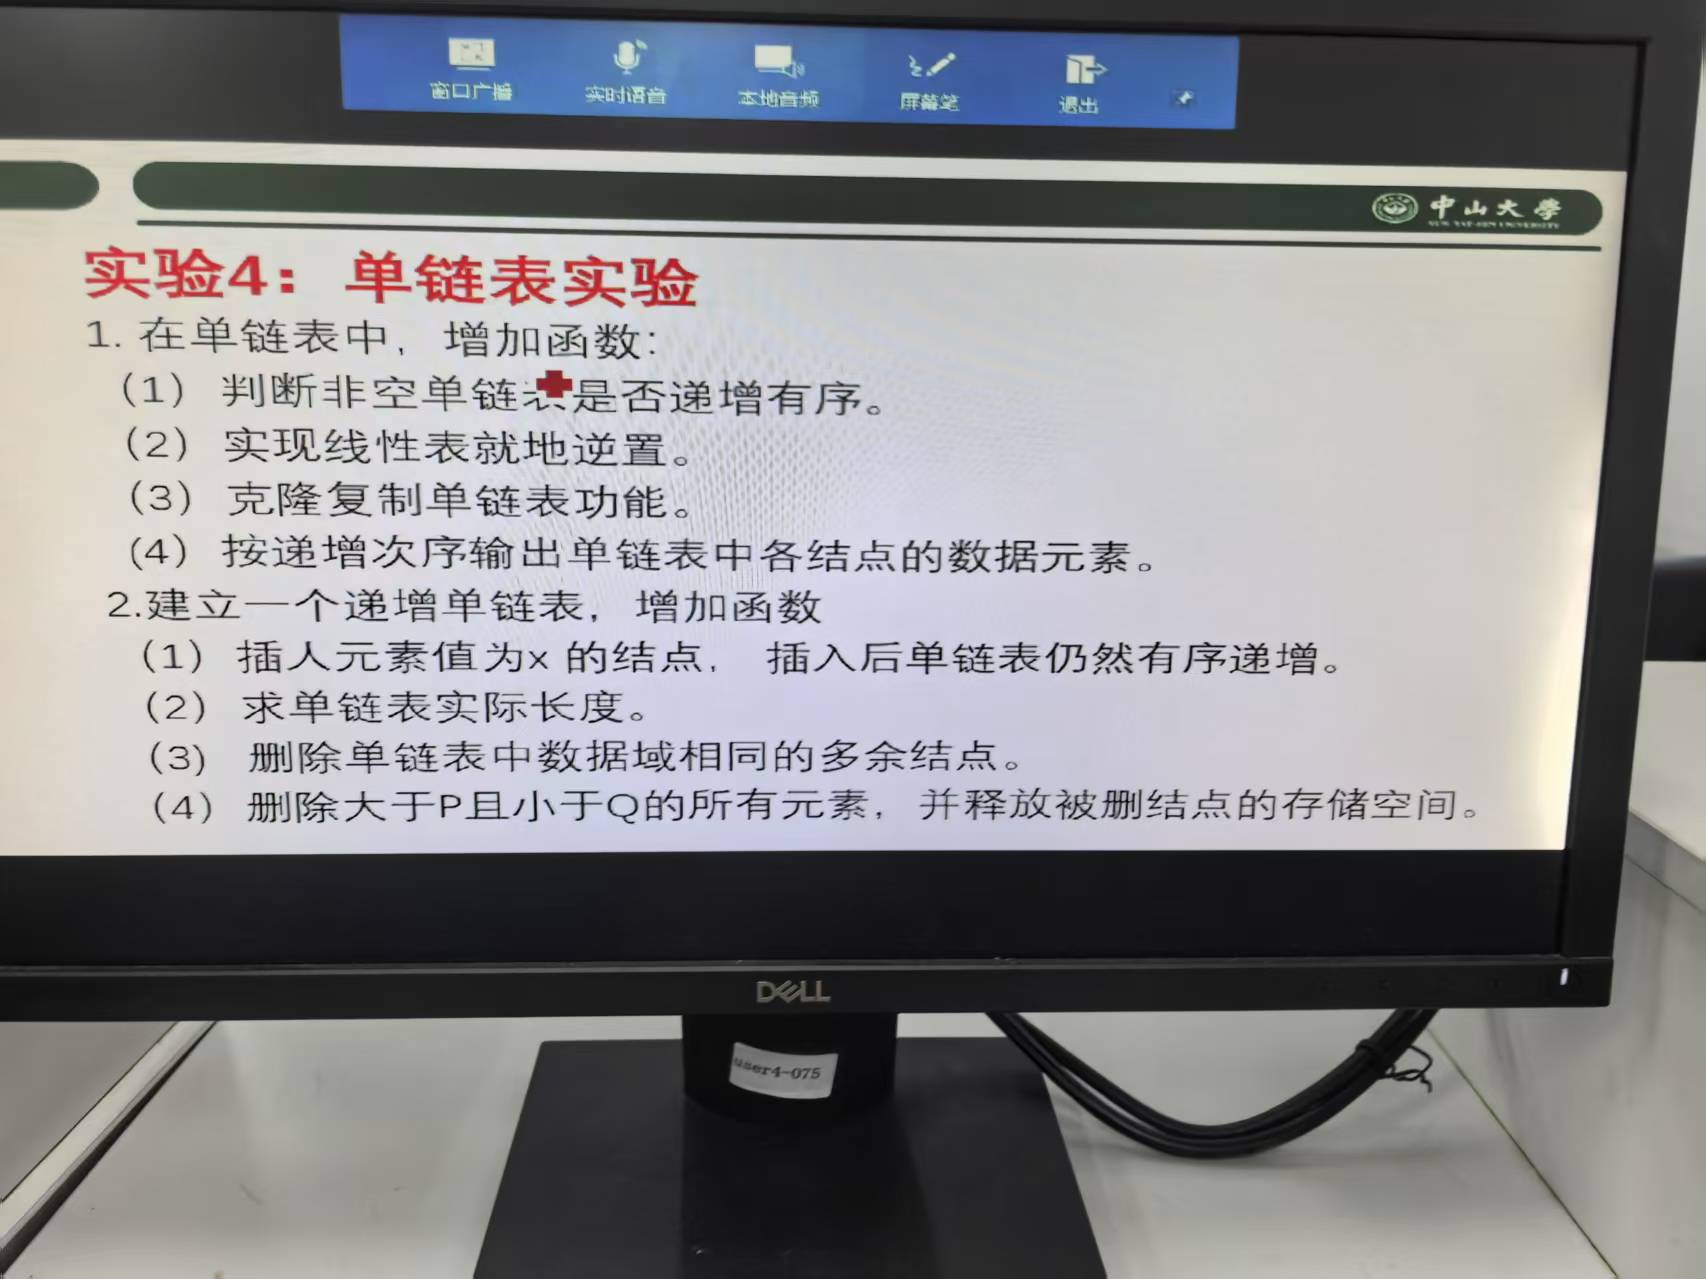
\includegraphics[width=\textwidth]{70b78d1af3cfcab6eb81c1ab96d2d22.jpg}
% \caption{}
\label{}
\end{figure}

\begin{figure}[H]
\centering
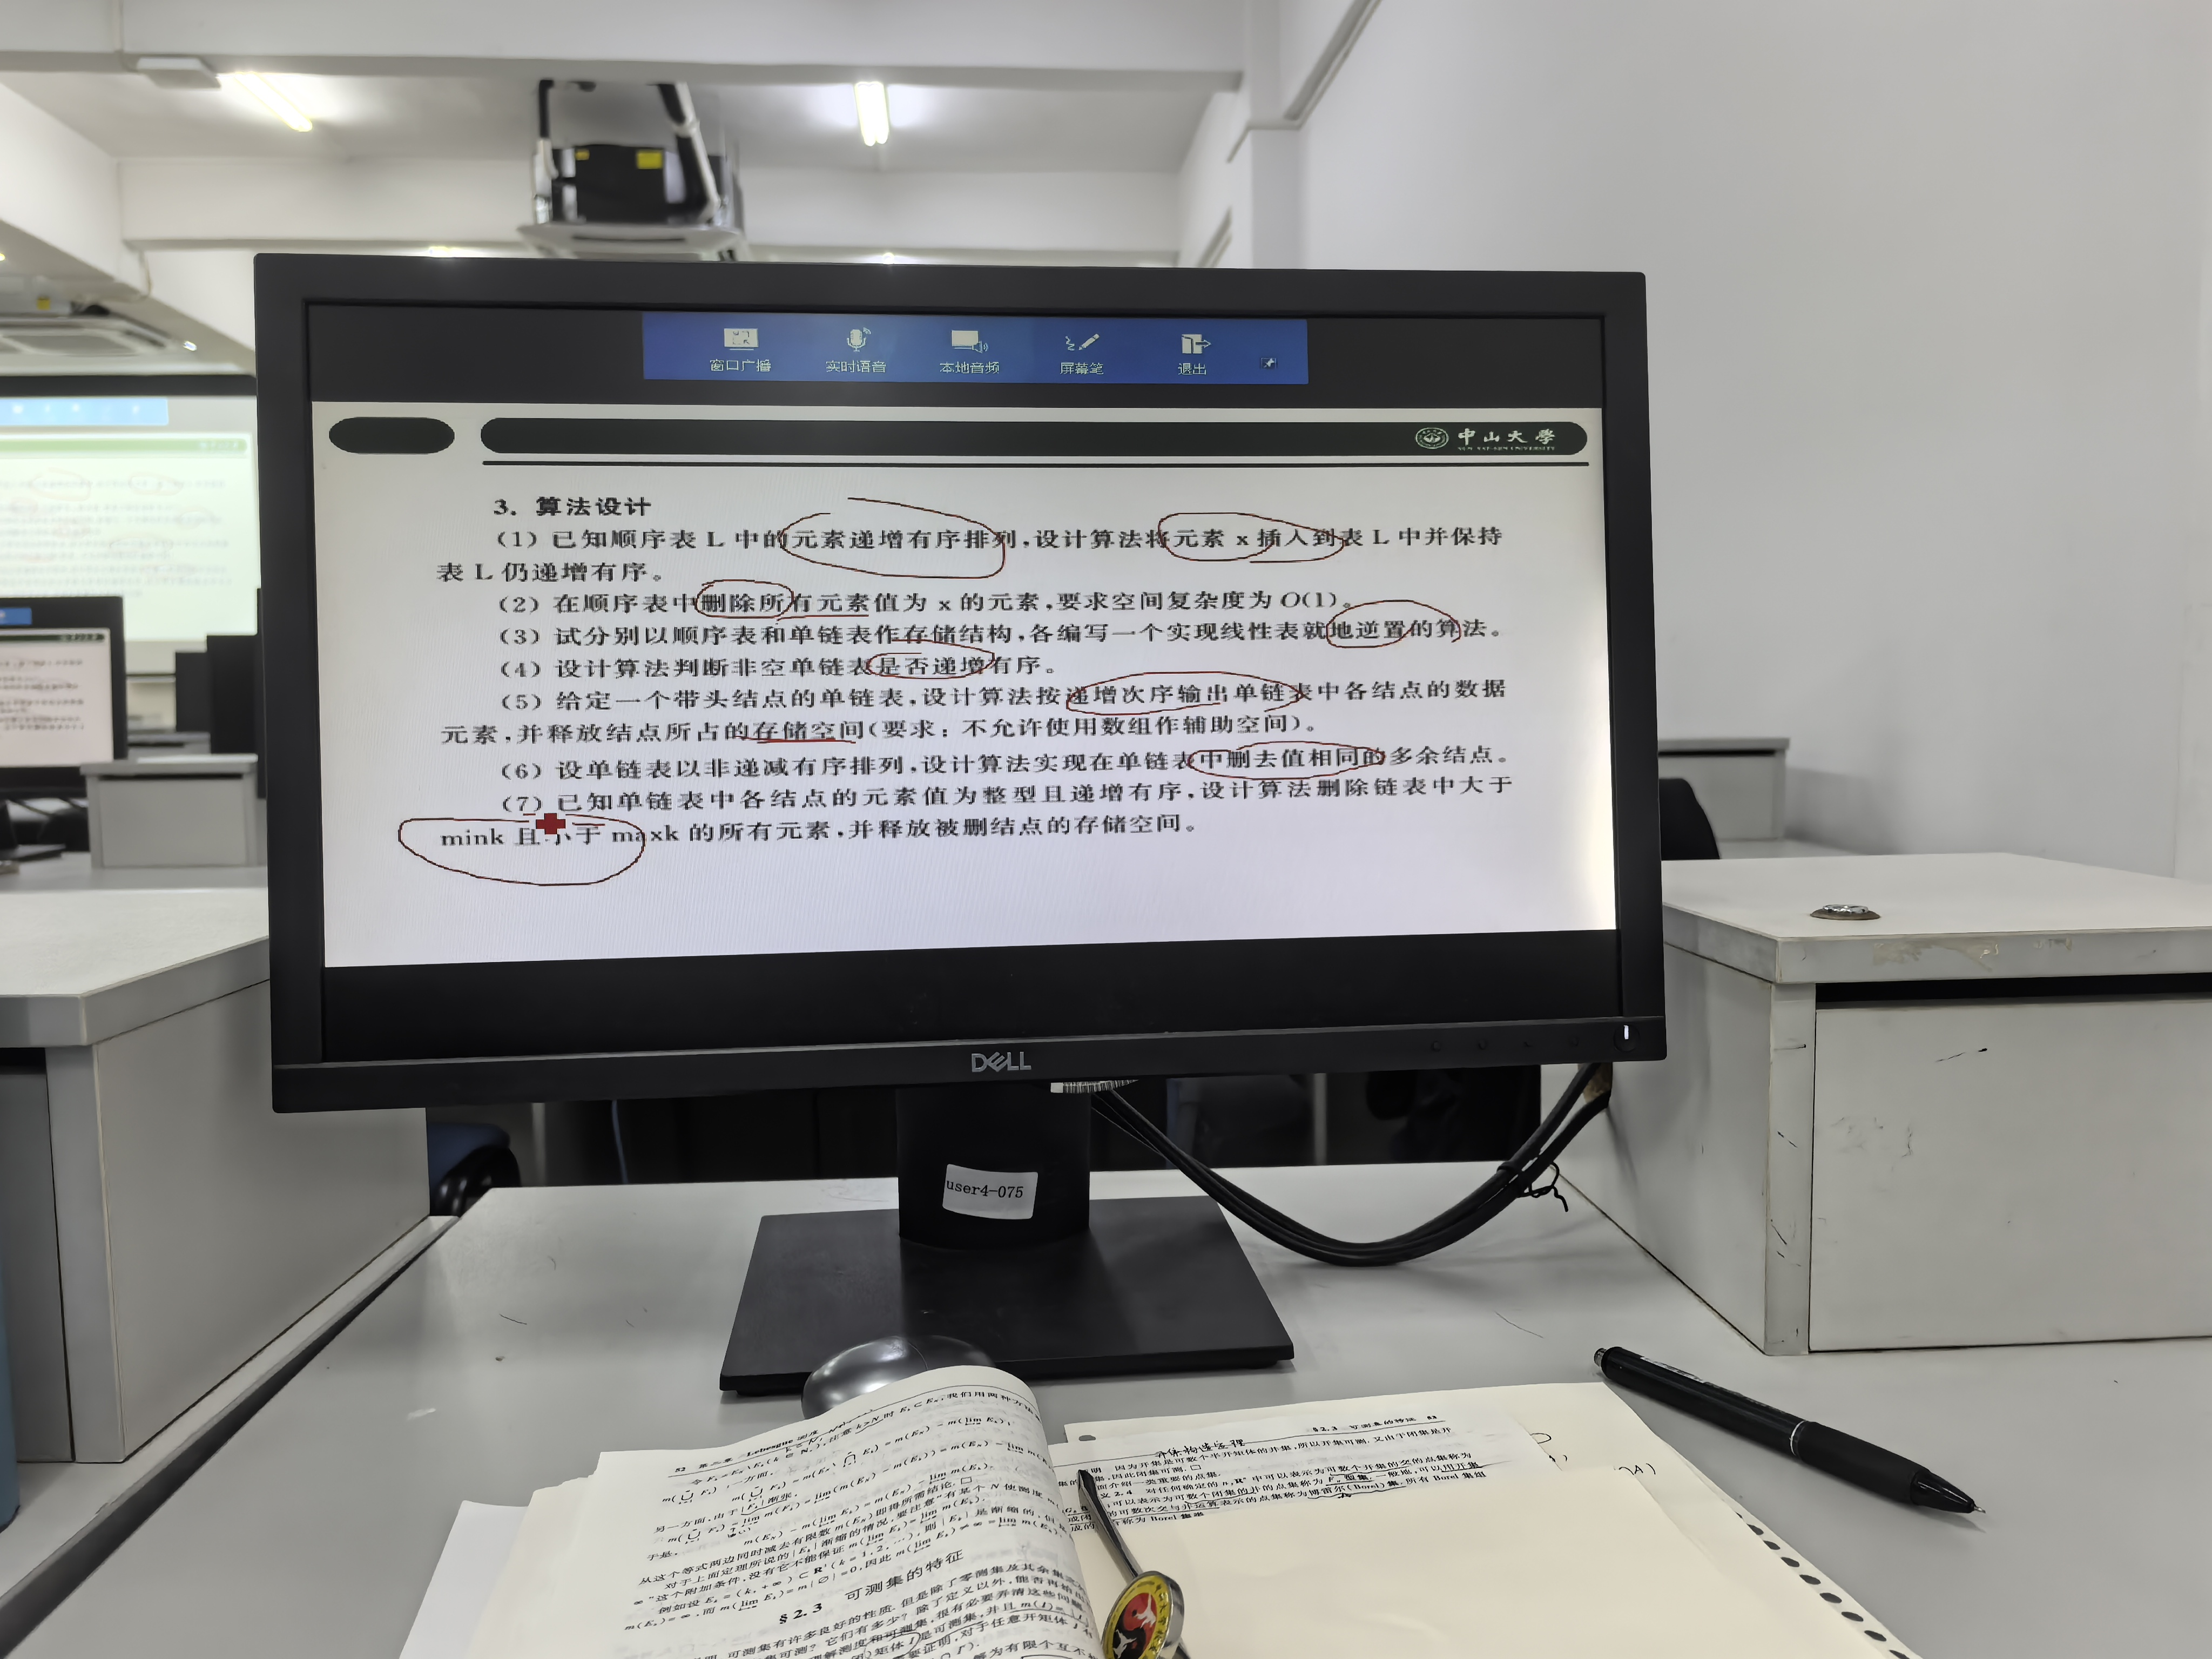
\includegraphics[width=\textwidth]{e676721f59bd9dd287376bd41486740.jpg}
% \caption{}
\label{}
\end{figure}

\section{题目 1}

\begin{figure}[H]
\centering
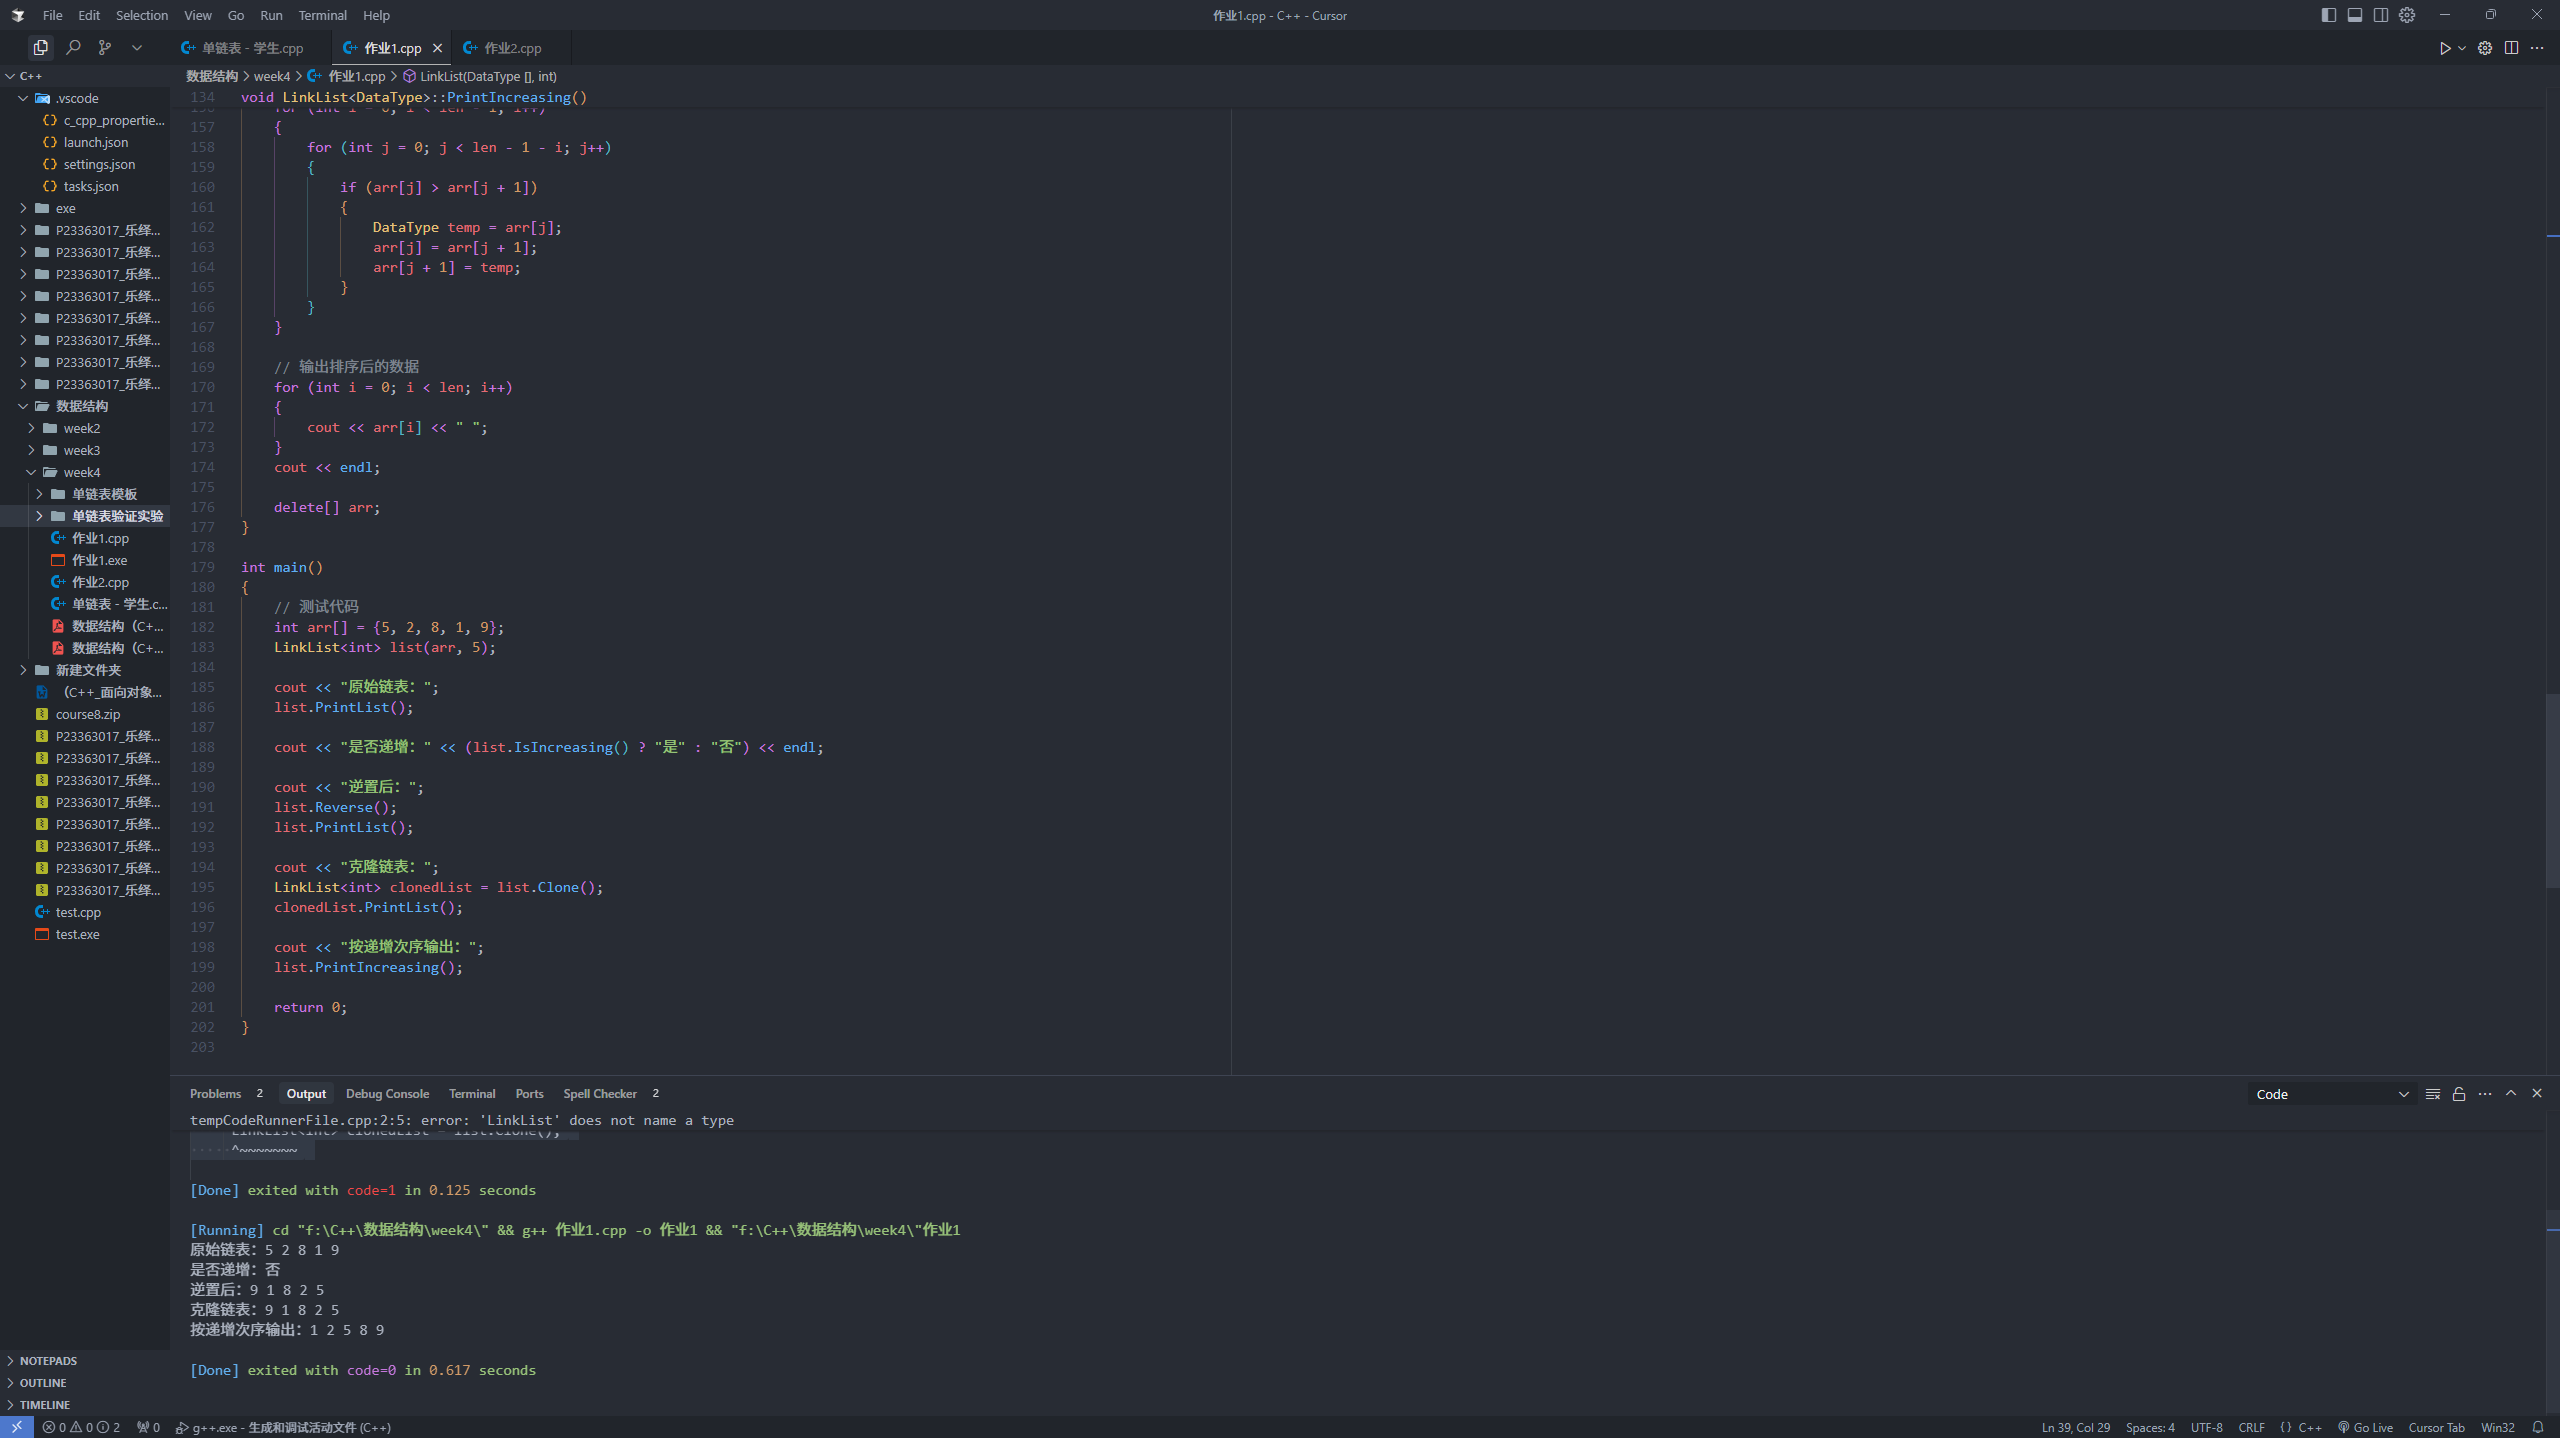
\includegraphics[width=\textwidth]{实验报告4-2025032418.png}
% \caption{}
\label{}
\end{figure}

\begin{lstlisting}[language=C++]
#include <iostream>

using namespace std;

  

template <typename DataType>

struct Node

{

    DataType data;               //数据域

    Node<DataType> *next;       //指针域

};

  

template <typename DataType>

class LinkList

{

public:

    LinkList();                      //无参构造函数,建立只有头结点的空链表

    LinkList(DataType a[], int n);   //有参构造函数,建立有n个元素的单链表

    ~LinkList();                     //析构函数

    void PrintList();                //遍历操作,按序号依次输出各元素

    // 新增功能

    bool IsIncreasing();             //判断是否为递增序列

    void Reverse();                  //就地逆置

    LinkList<DataType> Clone();      //克隆复制单链表

    void PrintIncreasing();          //按递增次序输出

  

private:

    Node<DataType> *first;          //单链表的头指针

};

  

// 构造函数

template <typename DataType>

LinkList<DataType>::LinkList()

{

    first = new Node<DataType>;

    first->next = NULL;

}

  

// 有参构造函数

template <typename DataType>

LinkList<DataType>::LinkList(DataType a[], int n)

{

    first = new Node<DataType>;

    first->next = NULL;

    Node<DataType> *r = first;

    for (int i = 0; i < n; i++)

    {

        Node<DataType> *s = new Node<DataType>;

        s->data = a[i];

        s->next = NULL;

        r->next = s;

        r = s;

    }

}

  

// 析构函数

template <typename DataType>

LinkList<DataType>::~LinkList()

{

    Node<DataType> *p = first;

    while (first != NULL)

    {

        first = first->next;

        delete p;

        p = first;

    }

}

  

// 打印链表

template <typename DataType>

void LinkList<DataType>::PrintList()

{

    Node<DataType> *p = first->next;

    while (p != NULL)

    {

        cout << p->data << " ";

        p = p->next;

    }

    cout << endl;

}

  

// 判断是否为递增序列

template <typename DataType>

bool LinkList<DataType>::IsIncreasing()

{

    if (first->next == NULL) return true;

    Node<DataType> *p = first->next;

    while (p->next != NULL)

    {

        if (p->data > p->next->data)

            return false;

        p = p->next;

    }

    return true;

}

  

// 就地逆置

template <typename DataType>

void LinkList<DataType>::Reverse()

{

    Node<DataType> *p = first->next;

    first->next = NULL;

    Node<DataType> *q;

    while (p != NULL)

    {

        q = p->next;

        p->next = first->next;

        first->next = p;

        p = q;

    }

}

  

// 克隆复制单链表

template <typename DataType>

LinkList<DataType> LinkList<DataType>::Clone()

{

    LinkList<DataType> newList;

    Node<DataType> *p = first->next;

    Node<DataType> *r = newList.first;

    while (p != NULL)

    {

        Node<DataType> *s = new Node<DataType>;

        s->data = p->data;

        s->next = NULL;

        r->next = s;

        r = s;

        p = p->next;

    }

    return newList;

}

  

// 按递增次序输出

template <typename DataType>

void LinkList<DataType>::PrintIncreasing()

{

    // 创建临时数组存储数据

    int len = 0;

    Node<DataType> *p = first->next;

    while (p != NULL)

    {

        len++;

        p = p->next;

    }

    DataType *arr = new DataType[len];

    p = first->next;

    // 复制数据到数组

    for (int i = 0; i < len; i++)

    {

        arr[i] = p->data;

        p = p->next;

    }

    // 冒泡排序

    for (int i = 0; i < len - 1; i++)

    {

        for (int j = 0; j < len - 1 - i; j++)

        {

            if (arr[j] > arr[j + 1])

            {

                DataType temp = arr[j];

                arr[j] = arr[j + 1];

                arr[j + 1] = temp;

            }

        }

    }

    // 输出排序后的数据

    for (int i = 0; i < len; i++)

    {

        cout << arr[i] << " ";

    }

    cout << endl;

    delete[] arr;

}

  

int main()

{

    // 测试代码

    int arr[] = {5, 2, 8, 1, 9};

    LinkList<int> list(arr, 5);

    cout << "原始链表:";

    list.PrintList();

    cout << "是否递增:" << (list.IsIncreasing() ? "是" : "否") << endl;

    cout << "逆置后:";

    list.Reverse();

    list.PrintList();

    cout << "克隆链表:";

    LinkList<int> clonedList = list.Clone();

    clonedList.PrintList();

    cout << "按递增次序输出:";

    list.PrintIncreasing();

    return 0;

}
\end{lstlisting}
\section{题目 2}

\begin{figure}[H]
\centering
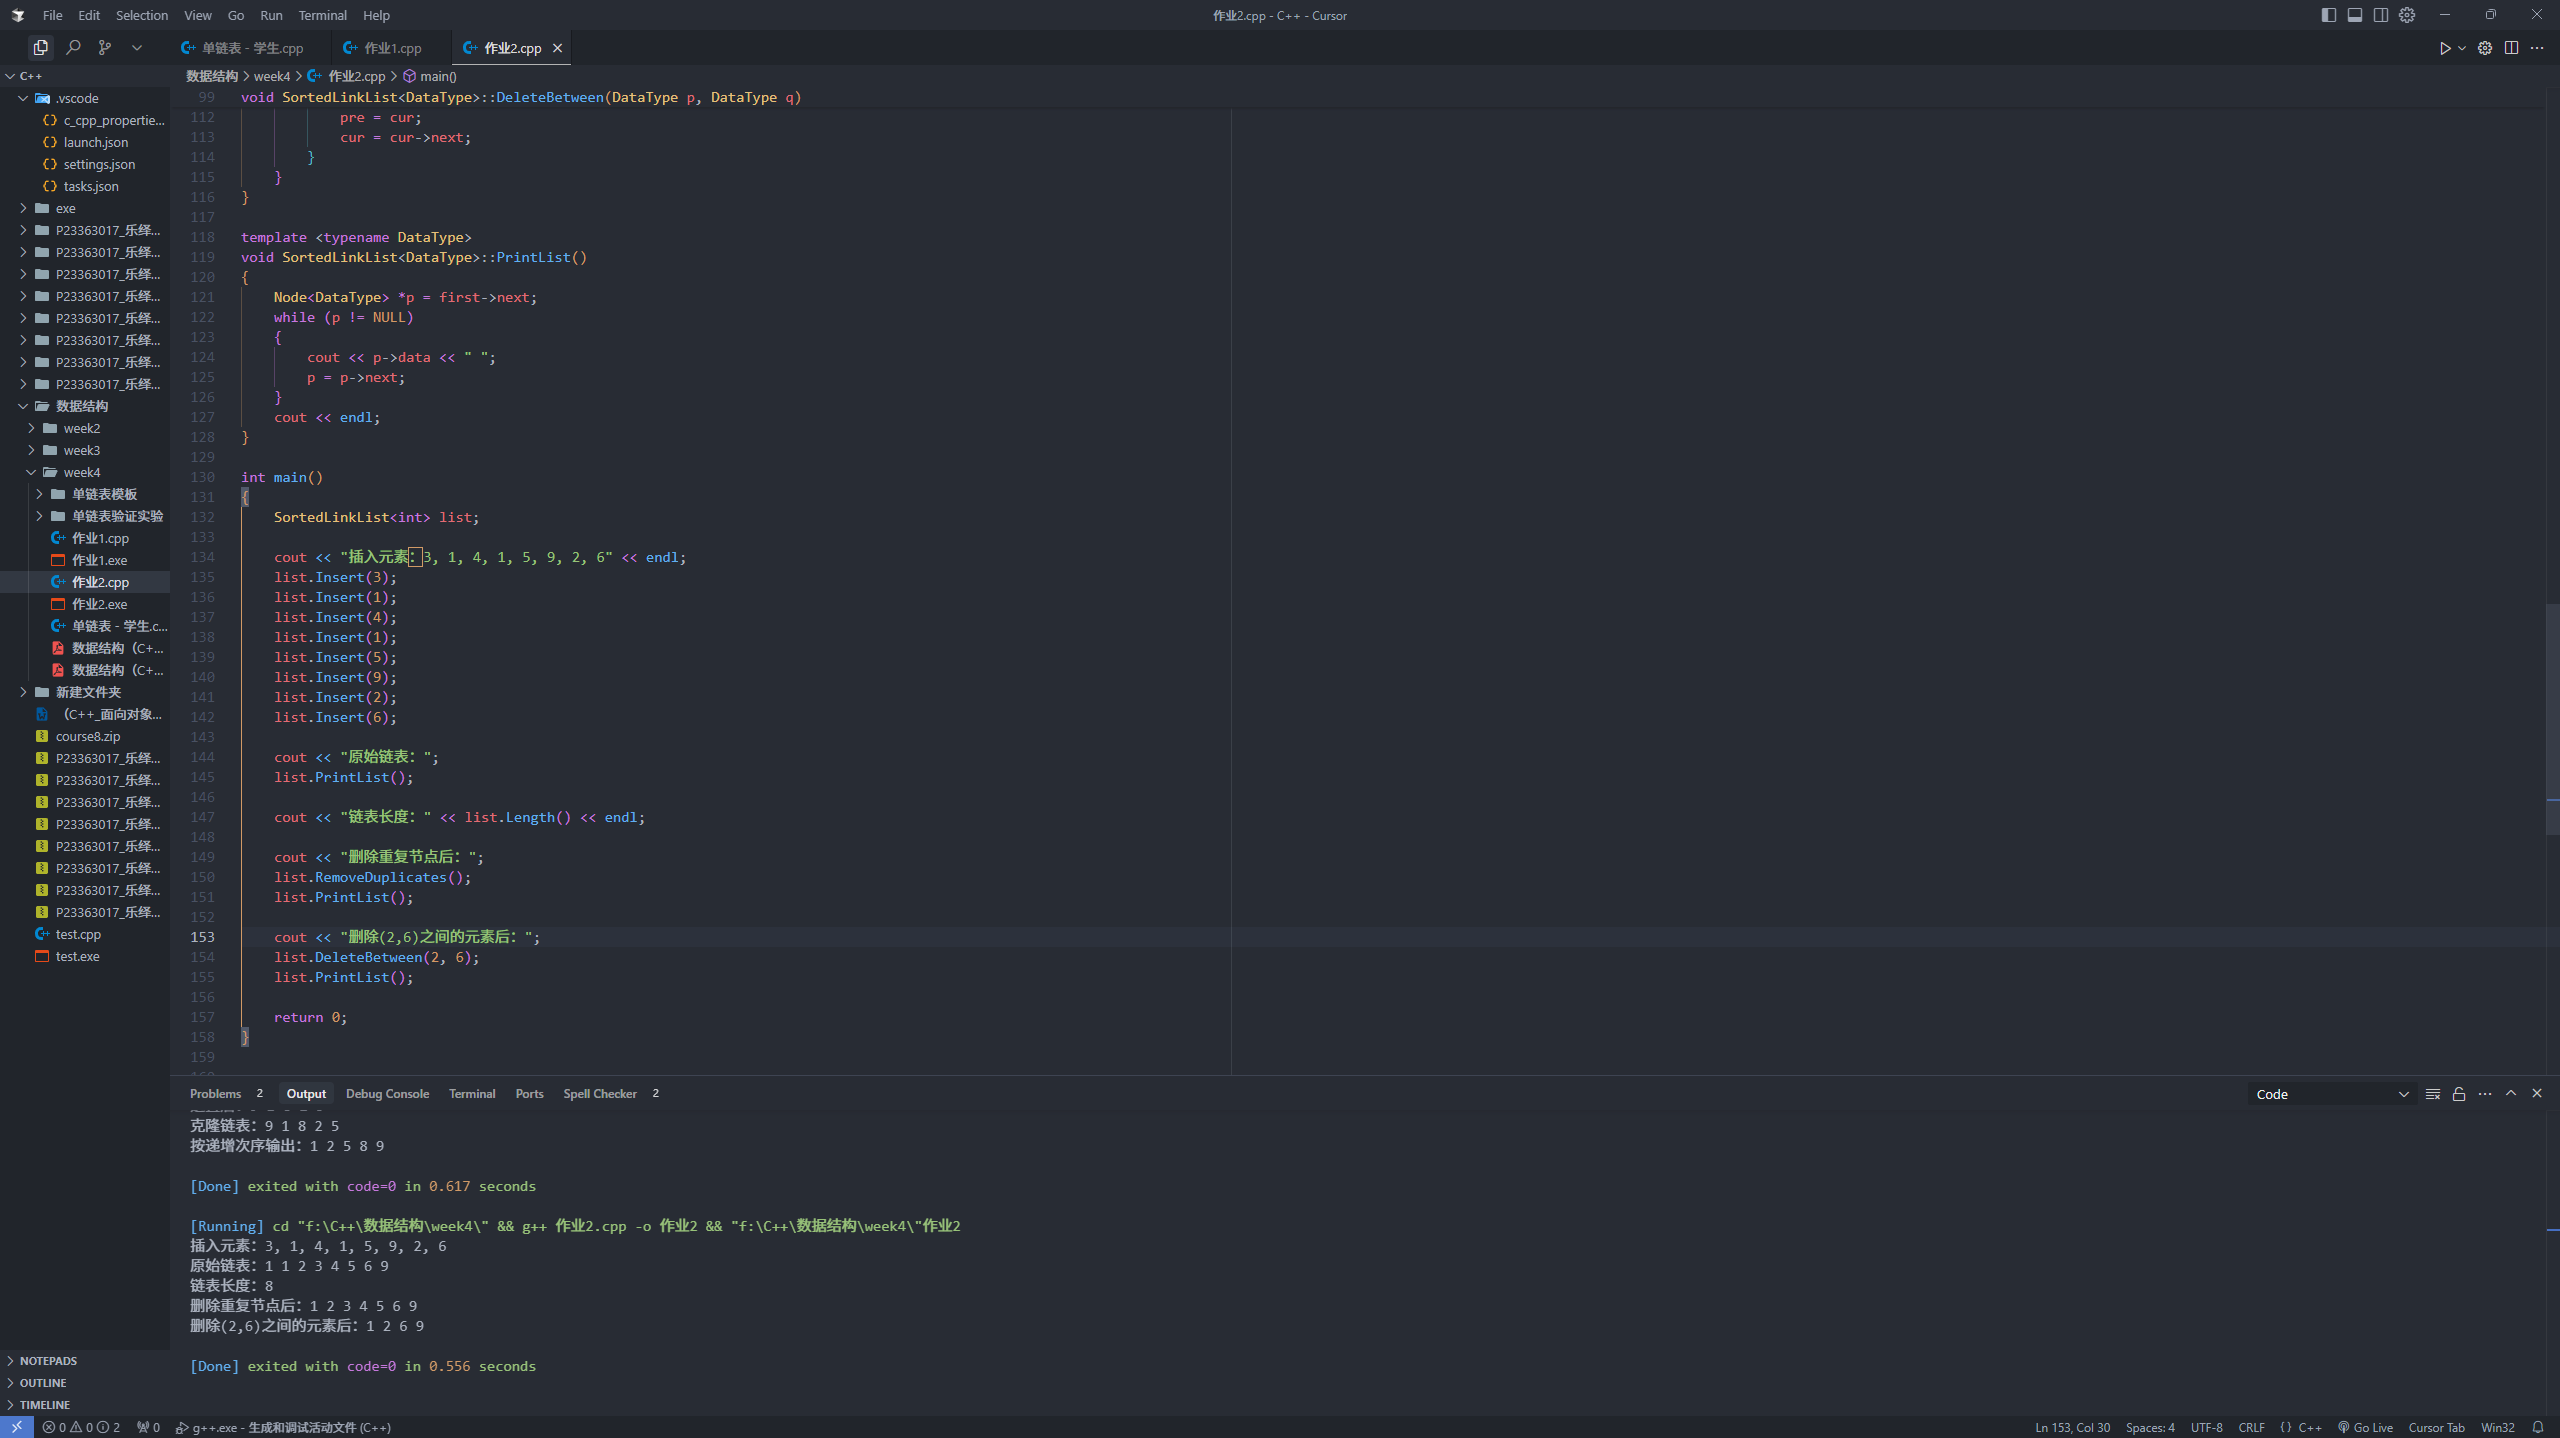
\includegraphics[width=\textwidth]{1-实验报告4-2025032418.png}
% \caption{}
\label{}
\end{figure}

\begin{lstlisting}[language=C++]
/*

2.建立一个递增单链表,增加函数

(1)插人元素值为×的结点,插入后单链表仍然有序递增。

(2)求单链表实际长度。

(3)删除单链表中数据域相同的多余结点。

(4)删除大于P且小于Q的所有元素,并释放被删结点的存储空间。

*/

#include <iostream>

using namespace std;

  

template <typename DataType>

struct Node

{

    DataType data;

    Node<DataType> *next;

};

  

template <typename DataType>

class SortedLinkList

{

public:

    SortedLinkList();

    ~SortedLinkList();

    void Insert(DataType x);

    int Length();

    void RemoveDuplicates();

    void DeleteBetween(DataType p, DataType q);

    void PrintList();

private:

    Node<DataType> *first;

};

  

template <typename DataType>

SortedLinkList<DataType> :: SortedLinkList()

{

    first = new Node<DataType>;

    first->next = NULL;

}  

  

template <typename DataType>

SortedLinkList<DataType> :: ~SortedLinkList()

{

    Node<DataType> *p = first;

    while (first != NULL)

    {  

        first = first->next;

        delete p;

        p = first;

    }

}

  

template <typename DataType>

void SortedLinkList<DataType>::Insert(DataType x)

{

    Node<DataType> *p = first;

    while (p->next != NULL && p->next->data < x)

    {

        p = p->next;

    }

    Node<DataType> *s = new Node<DataType>;

    s->data = x;

    s->next = p->next;

    p->next = s;

}

  

template <typename DataType>

int SortedLinkList<DataType>::Length()

{

    int count = 0;

    Node<DataType> *p = first->next;

    while (p != NULL)

    {

        count++;

        p = p->next;

    }

    return count;

}

  

template <typename DataType>

void SortedLinkList<DataType>::RemoveDuplicates()

{

    if (first->next == NULL || first->next->next == NULL) return;

    Node<DataType> *p = first->next;

    while (p != NULL && p->next != NULL)

    {

        if (p->data == p->next->data)

        {

            Node<DataType> *temp = p->next;

            p->next = p->next->next;

            delete temp;

        } else {

            p = p->next;

        }

    }

}

  

template <typename DataType>

void SortedLinkList<DataType>::DeleteBetween(DataType p, DataType q)

{

    Node<DataType> *pre = first;

    Node<DataType> *cur = first->next;

    while (cur != NULL)

    {

        if (cur->data > p && cur->data < q)

        {

            pre->next = cur->next;

            delete cur;

            cur = pre->next;

        } else {

            pre = cur;

            cur = cur->next;

        }

    }

}

  

template <typename DataType>

void SortedLinkList<DataType>::PrintList()

{

    Node<DataType> *p = first->next;

    while (p != NULL)

    {

        cout << p->data << " ";

        p = p->next;

    }

    cout << endl;

}

  

int main()

{

    SortedLinkList<int> list;

    cout << "插入元素:3, 1, 4, 1, 5, 9, 2, 6" << endl;

    list.Insert(3);

    list.Insert(1);

    list.Insert(4);

    list.Insert(1);

    list.Insert(5);

    list.Insert(9);

    list.Insert(2);

    list.Insert(6);

    cout << "原始链表:";

    list.PrintList();

    cout << "链表长度:" << list.Length() << endl;

    cout << "删除重复节点后:";

    list.RemoveDuplicates();

    list.PrintList();

    cout << "删除(2,6)之间的元素后:";

    list.DeleteBetween(2, 6);

    list.PrintList();

    return 0;

}
\end{lstlisting}
\section{题目 3}

\begin{figure}[H]
\centering
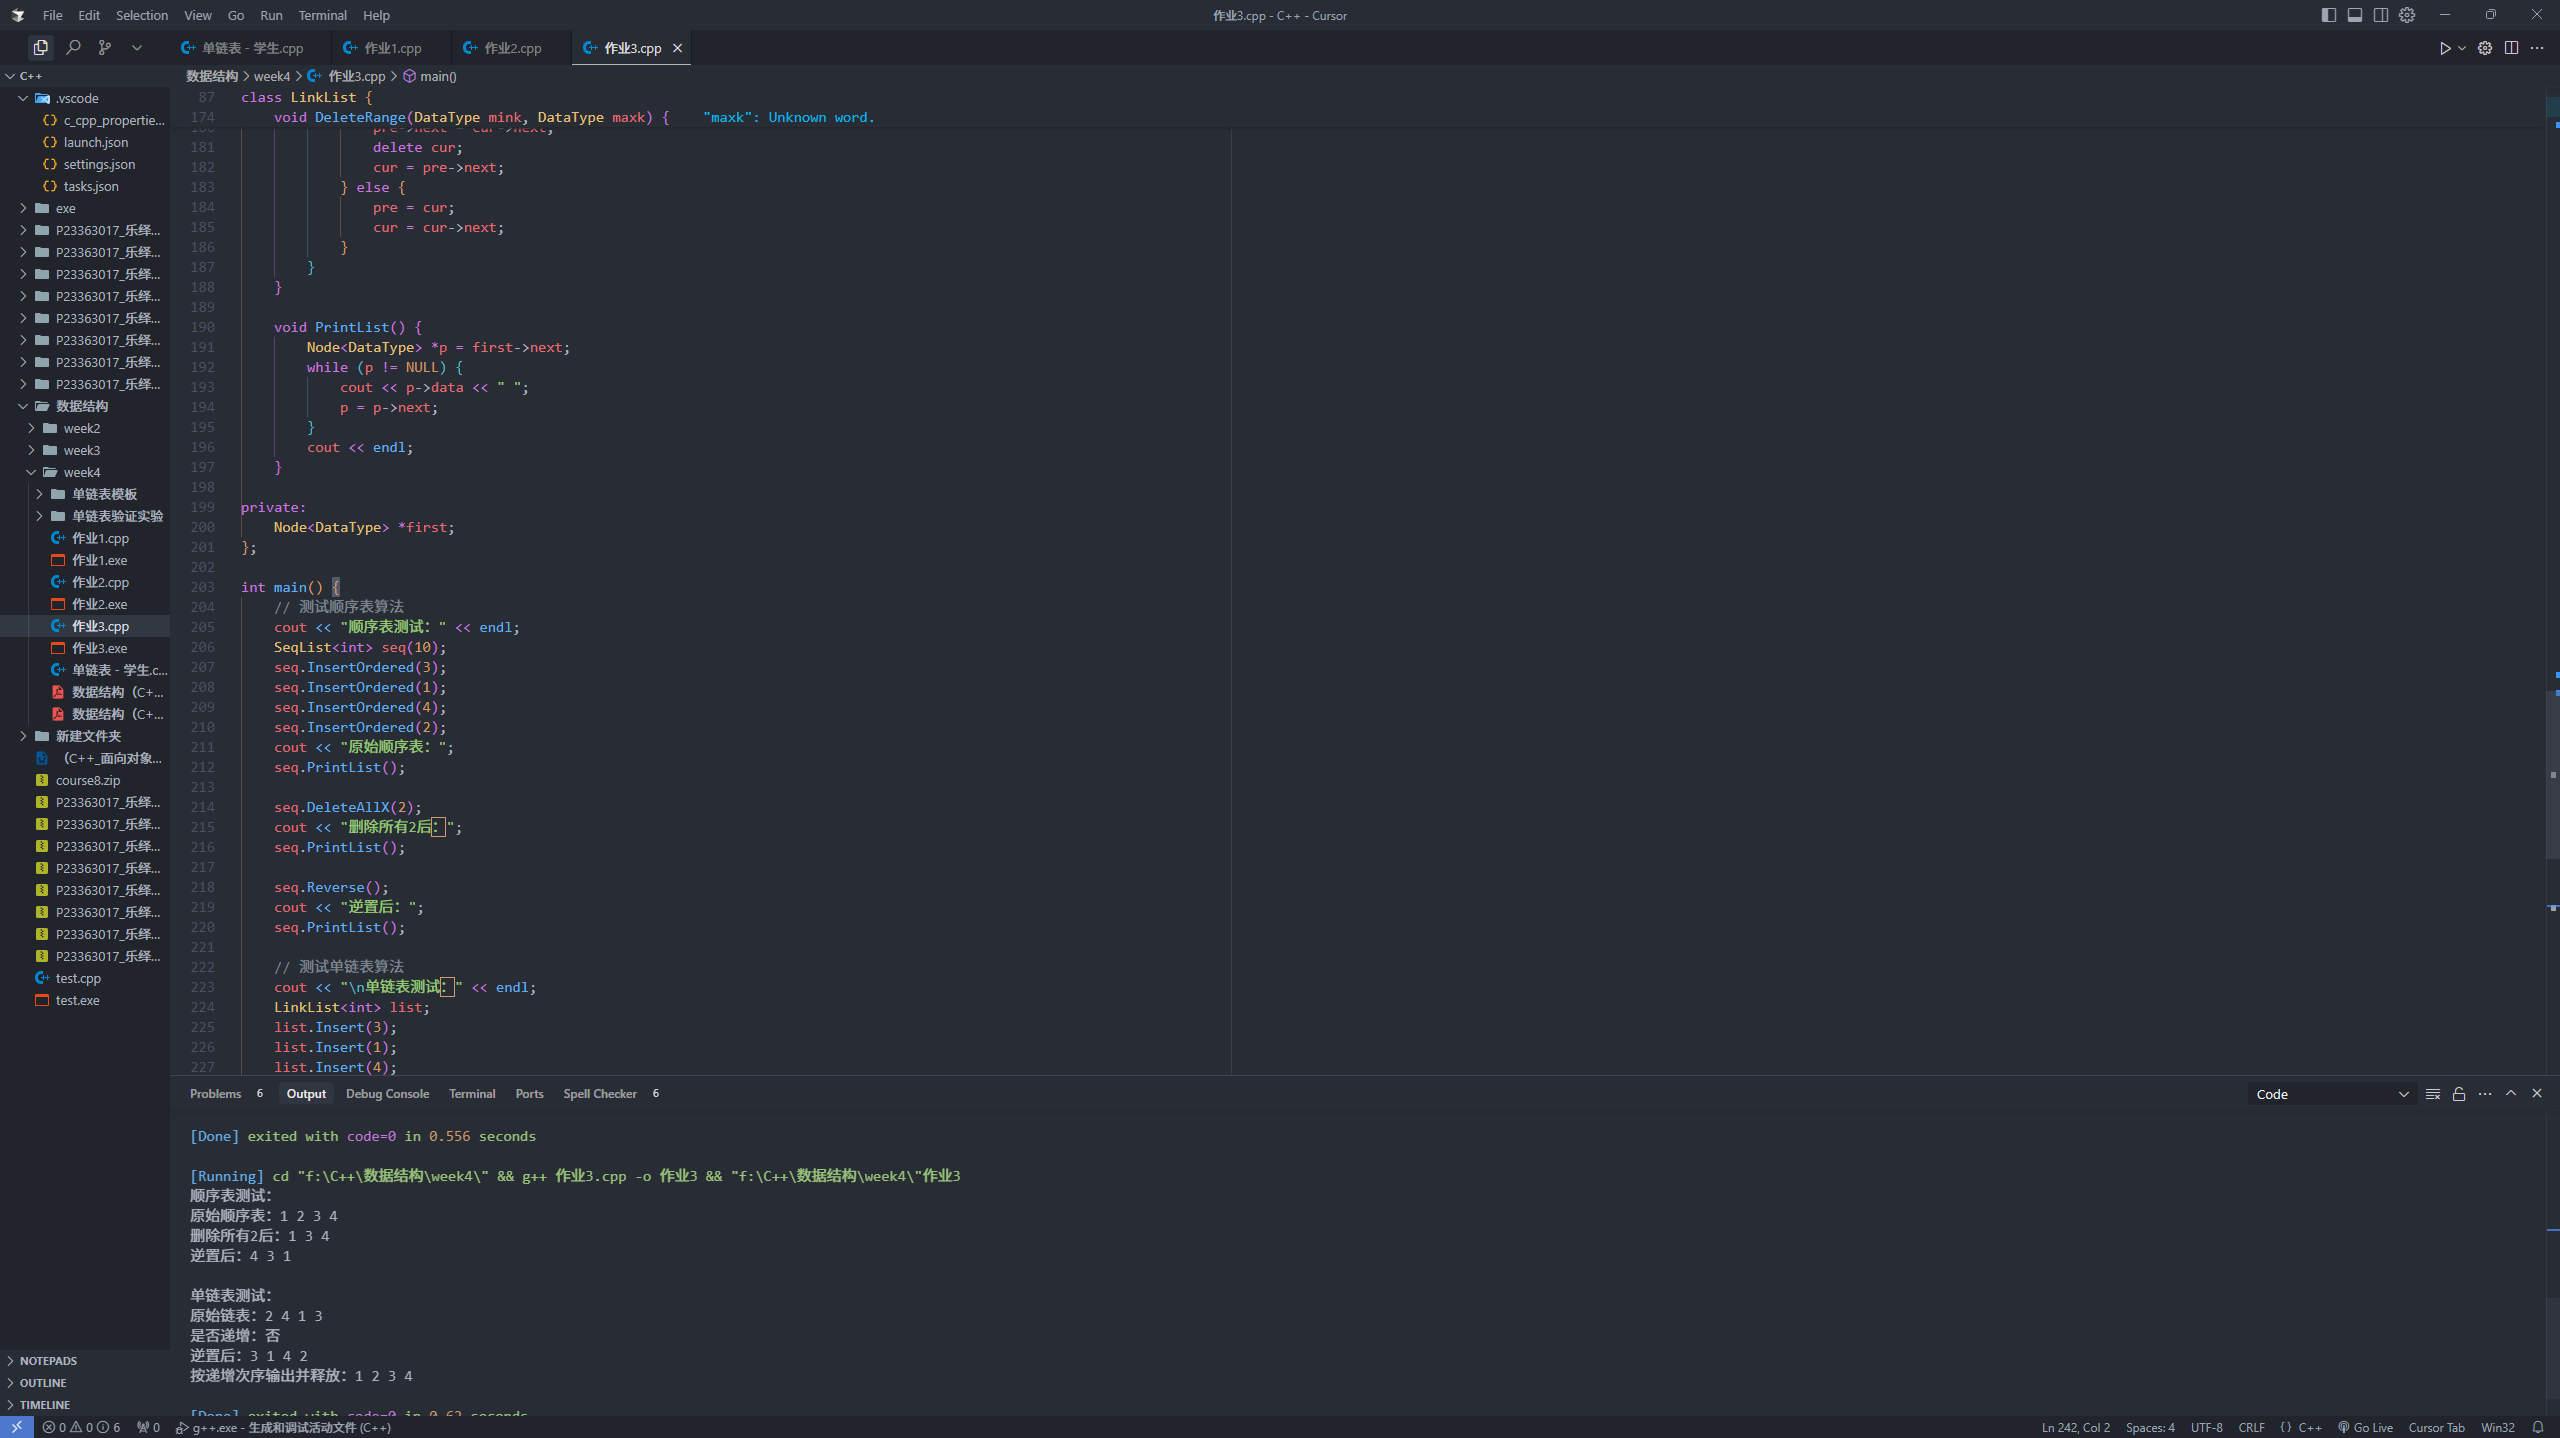
\includegraphics[width=\textwidth]{实验报告4-2025032419.png}
% \caption{}
\label{}
\end{figure}

\begin{lstlisting}[language=C++]
/*

3.算法设计

(1)已知顺序表L中的元素递增有序排列,设计算法将元素x插人到表L中并保持

表L仍递增有序。

(2)在顺序表中删除所有元素值为x的元素,要求空间复杂度为0(1)

(3)试分别以顺序表和单链表作存储结构,各编写一个实现线性表就地逆置的算法。

(4)设计算法判断非空单链表是否递增有序。

(5)给定一个带头结点的单链表,设计算法按递增次序输出单链表中各结点的数据

元素,并释放结点所占的存储空间(要求:不允许使用数组作辅助空间)。

(6)设单链表以非递减有序排列,设计算法实现在单链表中删去值相同的多余结点。

(7)已知单链表中各结点的元素值为整型且递增有序,设计算法删除链表中大于

mink且于maxk的所有元素,并释放被删结点的存储空间。

*/

  

#include <iostream>

using namespace std;

  

// 顺序表类

template <typename DataType>

class SeqList {

public:

    SeqList(int size = 100) {

        maxSize = size;

        length = 0;

        data = new DataType[maxSize];

    }

    ~SeqList() {

        delete[] data;

    }

    // (1) 在递增有序顺序表中插入元素x

    void InsertOrdered(DataType x) {

        if (length >= maxSize) throw "上溢";

        int i;

        // 找到插入位置

        for (i = 0; i < length && data[i] <= x; i++);

        // 将元素后移

        for (int j = length; j > i; j--) {

            data[j] = data[j-1];

        }

        data[i] = x;

        length++;

    }

    // (2) 删除所有值为x的元素,空间复杂度O(1)

    void DeleteAllX(DataType x) {

        int k = 0;  // k记录不等于x的元素个数

        for (int i = 0; i < length; i++) {

            if (data[i] != x) {

                data[k] = data[i];

                k++;

            }

        }

        length = k;

    }

    // (3) 顺序表就地逆置

    void Reverse() {

        for (int i = 0; i < length/2; i++) {

            DataType temp = data[i];

            data[i] = data[length-1-i];

            data[length-1-i] = temp;

        }

    }

    void PrintList() {

        for (int i = 0; i < length; i++) {

            cout << data[i] << " ";

        }

        cout << endl;

    }

private:

    DataType *data;

    int maxSize;

    int length;

};

  

// 单链表类

template <typename DataType>

struct Node {

    DataType data;

    Node<DataType> *next;

};

  

template <typename DataType>

class LinkList {

public:

    LinkList() {

        first = new Node<DataType>;

        first->next = NULL;

    }

    ~LinkList() {

        Node<DataType> *p = first;

        while (first != NULL) {

            first = first->next;

            delete p;

            p = first;

        }

    }

    // 插入元素

    void Insert(DataType x) {

        Node<DataType> *s = new Node<DataType>;

        s->data = x;

        s->next = first->next;

        first->next = s;

    }

    // (3) 单链表就地逆置

    void Reverse() {

        Node<DataType> *p = first->next;

        first->next = NULL;

        Node<DataType> *q;

        while (p != NULL) {

            q = p->next;

            p->next = first->next;

            first->next = p;

            p = q;

        }

    }

    // (4) 判断是否递增有序

    bool IsIncreasing() {

        if (first->next == NULL) return true;

        Node<DataType> *p = first->next;

        while (p->next != NULL) {

            if (p->data > p->next->data) return false;

            p = p->next;

        }

        return true;

    }

    // (5) 按递增次序输出并释放空间

    void PrintAndFree() {

        while (first->next != NULL) {

            // 找到最小值节点

            Node<DataType> *minPrev = first;

            Node<DataType> *p = first->next;

            Node<DataType> *minNode = p;

            while (p->next != NULL) {

                if (p->next->data < minNode->data) {

                    minPrev = p;

                    minNode = p->next;

                }

                p = p->next;

            }

            // 输出并删除最小值节点

            cout << minNode->data << " ";

            minPrev->next = minNode->next;

            delete minNode;

        }

        cout << endl;

    }

    // (6) 删除值相同的多余节点

    void RemoveDuplicates() {

        if (first->next == NULL || first->next->next == NULL) return;

        Node<DataType> *p = first->next;

        while (p != NULL && p->next != NULL) {

            if (p->data == p->next->data) {

                Node<DataType> *temp = p->next;

                p->next = p->next->next;

                delete temp;

            } else {

                p = p->next;

            }

        }

    }

    // (7) 删除大于mink且小于maxk的元素

    void DeleteRange(DataType mink, DataType maxk) {

        Node<DataType> *pre = first;

        Node<DataType> *cur = first->next;

        while (cur != NULL) {

            if (cur->data > mink && cur->data < maxk) {

                pre->next = cur->next;

                delete cur;

                cur = pre->next;

            } else {

                pre = cur;

                cur = cur->next;

            }

        }

    }

    void PrintList() {

        Node<DataType> *p = first->next;

        while (p != NULL) {

            cout << p->data << " ";

            p = p->next;

        }

        cout << endl;

    }

private:

    Node<DataType> *first;

};

  

int main() {

    // 测试顺序表算法

    cout << "顺序表测试:" << endl;

    SeqList<int> seq(10);

    seq.InsertOrdered(3);

    seq.InsertOrdered(1);

    seq.InsertOrdered(4);

    seq.InsertOrdered(2);

    cout << "原始顺序表:";

    seq.PrintList();

    seq.DeleteAllX(2);

    cout << "删除所有2后:";

    seq.PrintList();

    seq.Reverse();

    cout << "逆置后:";

    seq.PrintList();

    // 测试单链表算法

    cout << "\n单链表测试:" << endl;

    LinkList<int> list;

    list.Insert(3);

    list.Insert(1);

    list.Insert(4);

    list.Insert(2);

    cout << "原始链表:";

    list.PrintList();

    cout << "是否递增:" << (list.IsIncreasing() ? "是" : "否") << endl;

    list.Reverse();

    cout << "逆置后:";

    list.PrintList();

    cout << "按递增次序输出并释放:";

    list.PrintAndFree();

    return 0;

}
\end{lstlisting}